% THIS IS GDANSK UNIVERSITY OF TECHNLOGOGY (PG) PRESENTATION TEMPLATE
% Creator: Jan Cychnerski <jan.cychnerski@eti.pg.edu.pl>
% Copyleft 2019

% traditional screen
\documentclass{beamer}

% wide screen
%\documentclass[aspectratio=169]{beamer}


%%% YOUR PACKAGES HERE %%%
\usepackage{comment}
\usepackage{hyperref}
\usepackage{graphicx}
\usepackage{wrapfig}


% polish language
\usepackage[polish]{babel}
\usepackage{polski}



%%% IMPORT PG PRESENTATION STYLE %%%
\include{pgbeamer/pgbeamer}



%%% YOUR OPTIONS HERE %%%

\title[Równania Naviera-Stokesa w fizyce i technice]{Równania Naviera-Stokesa w fizyce i technice}
\subtitle{WFTiMS: Fizyka Techniczna\\ III rok, VI semestr: Fizyka Stosowana}
\author{Andrei Hileuski}
\date{14.IV.2026}

%\setbeamercovered{transparent}





%%% DOCUMENT BEGINS HERE %%%

\begin{document}

%%% PG TITLE PAGE %%%
\pgtitleframe

%%% YOUR PRESENTATION HERE %%%


\begin{frame}{Plan prezentacji}
	\begin{itemize}
		\item Podstawy mechaniki płynów
		\item "Wyprowadzenie"
		\item Równania Naviera-Stokesa
		\item Szczególne przypadki
		\item Zastosowania
		\item Podsumowanie
		\item Źródła
	\end{itemize}
\end{frame}

\begin{frame}{Podstawy mechaniki płynów 1}
	Wspómnimy równania Eulera i ciągłości dla płynu nieściśliwego i nielepkiego:


	\begin{equation}
		\frac{D\textbf{u}}{Dt} = \frac{\partial \textbf{u}}{\partial t} + (\textbf{u} \cdot \nabla) \textbf{u} = -\frac{\nabla p}{\rho} + \textbf{g}
		\label{eq:euler0}
	\end{equation}

	
	\begin{equation}
		\nabla \cdot \textbf{u} = 0
		\label{eq:incompressibility}
	\end{equation}


	
	\begin{equation}
		\frac{\partial \rho}{\partial t} +
		\nabla \cdot (\rho \textbf{u}) = 0
		\label{eq:continuity}
	\end{equation}
	

	Równanie Eulera w formie tensorowej (zaniedbując siły zewnętrzne \textbf{g}):

	\begin{equation}
		\frac{\partial u_i}{\partial t} = -u_k \frac{\partial u_i}{\partial x_k}
		-\frac{1}{\rho} \frac{\partial p}{\partial x_i}
		\label{eq:euler_tensor}
	\end{equation}

\end{frame}

\begin{frame}{Podstawy mechaniki płynów 2}
	
	Szybkość zmiany pędu:

	
	\begin{equation}
		\frac{\partial}{\partial t} \rho\textbf{u}
		\label{eq:vector_ped}
	\end{equation}

	
	\begin{equation}
		\frac{\partial}{\partial t}\rho u_i = \rho\ \frac{\partial u_i}{\partial t}
		+ u_i\ \frac{\partial \rho}{\partial t}
		\label{eq:ped_tensor}
	\end{equation}


	Człon $\frac{\partial\rho}{\partial t}$ można wziąć z równania ciągłości
	\eqref{eq:continuity} i człon $\frac{\partial u_i}{\partial t}$
	można wziąć z równania Eulera \eqref{eq:euler_tensor}:

	\begin{equation}
		\frac{\partial\rho}{\partial t} = -\frac{\partial(\rho u_k)}{\partial x_k}
		\label{eq:continuity_tensor}
	\end{equation}

	\begin{equation}
		\frac{\partial u_i}{\partial t} = -u_k\ \frac{\partial u_i}{\partial x_k}
		-\frac{1}{\rho}\ \frac{\partial p}{\partial x_i}
		\label{eq:euler_tensor2}
	\end{equation}


\end{frame}

\begin{frame}{Podstawy mechaniki płynów 3}
	Wtedy z wyrazów \eqref{eq:ped_tensor}-\eqref{eq:euler_tensor2} mamy:

	\begin{equation}
		\frac{\partial}{\partial t} \rho u_i =
		-\rho u_k \frac{\partial u_i}{\partial x_k}
		-\frac{\partial p}{\partial x_i}
		-u_i \frac{\partial (\rho u_k)}{\partial x_k}
		=-\frac{\partial p}{\partial x_i} -
		\frac{\partial}{\partial x_k}\rho u_i u_k
		\label{eq:ped_tensor2}
	\end{equation}

	Człon $\frac{\partial p}{\partial x_i}$ można zapisać jako:

	\begin{equation}
		\frac{\partial p}{\partial x_i} =
		\delta_{ik} \frac{\partial p}{\partial x_k}
		\label{eq:press_delta}
	\end{equation}

	I z powyższych wzorów \eqref{eq:ped_tensor2}-\eqref{eq:press_delta} mamy:

	\begin{equation}
		\frac{\partial}{\partial t} \rho u_i =
		-\frac{\partial \Pi_{ik}}{\partial x_k}
		\label{eq:ped_tensor3}
	\end{equation}

	gdzie $\Pi_{ik}$ (tzw. tensor strumienia pędu) jest dany wzorem:

	\begin{equation}
		\Pi_{ik} = p \delta_{ik} + \rho u_i u_k
		\label{eq:momentum_flux}
	\end{equation}

\end{frame}

\begin{frame}{Podstawy mechaniki płynów 4}

	Wyjaśnić sens tensora $\Pi$ można obustronnie całkując równanie
	\eqref{eq:ped_tensor3} po objętosci $dV$:

	\begin{equation}
		\frac{\partial}{\partial t} \int \rho u_i dV =
		-\int \frac{\partial \Pi_{ik}}{\partial x_k} dV
	\label{eq:ped_integral}
	\end{equation}

	\begin{equation}
		\frac{\partial}{\partial t} \int \rho u_i dV =
		-\oint \Pi_{ik} n_k dS
	\label{eq:ped_integral2}
	\end{equation}
\end{frame}

\begin{frame}{"Wyprowadzenie"}
	Modyfikowany tensor strumienia pędu dla płynu lepkościowego:
	\begin{equation}
		\Pi_{ik} = p\delta_{ik} + \rho u_i u_k - \sigma'_{ik} = 
		-\sigma_{ik} + \rho u_i u_k
		\label{eq:momentum_flux_viscous}
	\end{equation}

	\begin{equation}
		\sigma_{ik} = -p\delta_{ik} + \sigma'_{ik}
		\label{eq:stress_tensor_viscous}
	\end{equation}

	Gdzie $\sigma_{ik}$ jest tzw. temsorem naprężeń, 
	a $\sigma'_{ik}$ jest tzw. tensorem naprężeń lepkościowych.

	\begin{figure}[ht]
		\centering
		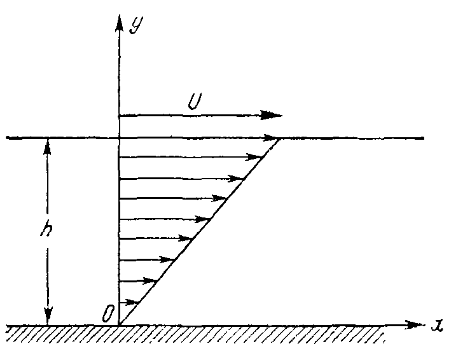
\includegraphics[width=0.275\textwidth]{figures/visc_fluid.png}
		\caption{Model płynu lepkościowego. Źródło:N.E. Kochin, I.A. Kibel --
		"Teoreticheskaya gidrodinamika" ch.2, Moskva Fizmatlit, 1963}
		\label{fig:visc_fluid}
	\end{figure}

\end{frame}

\begin{frame}{"Wyprowadzenie"}
	Czyli temsor lepkościowy musi zaweirać:

	\begin{equation}
		\frac{\partial u_i}{\partial x_k} + \frac{\partial u_k}{\partial x_i}
	\label{eq:velocity_rotation}
	\end{equation}

	Najczęściej przyjmuje się następna postać tensora lepkościowego:

	\begin{equation}
		\sigma'{ik} = \eta \left( \frac{\partial u_i}{\partial x_k} +
		\frac{\partial u_k}{\partial x_i} - \frac{2}{3}\delta_{ik}
		\frac{\partial u_l}{\partial x_l} \right) + 
		\zeta \delta_{ik} \frac{\partial u_l}{\partial x_l}
	\label{eq:viscous_stress_tensor}
	\end{equation}

	Gdzie lepkość dynamiczna $\eta$ i lepkość objętościowa 
	$\zeta$ muszą być dodatnie:

	\begin{equation}
		\eta, \zeta > 0
	\end{equation}
\end{frame}

\begin{frame}{"Wyprowadzenie"}

	Równania Eulera \eqref{eq:euler_tensor} można zapisać jako:

	\begin{equation}
		\rho \left(\frac{u_i}{t} + u_k
		\frac{\partial u_i}{\partial x_k}\right) =
		-\frac{\partial p}{\partial x_i}
	\label{eq:euler_tensor3}
	\end{equation}

	I ze wzorów \eqref{eq:ped_tensor3}, \eqref{eq:momentum_flux_viscous},
	\eqref{eq:stress_tensor_viscous} wynika, że równania
	ruchu dla lepkiego płynu można otrzymać dodając człon
	$\frac{\partial \sigma'_{ik}}{\partial x_k}$ do prawej strony równania
	\eqref{eq:euler_tensor3}:

	\begin{equation}
		\begin{split}
		\rho \left(\frac{\partial u_i}{\partial t} + 
		u_k \frac{\partial u_i}{\partial x_k}\right) & =
		-\frac{\partial p}{\partial x_i} +
		\frac{\partial}{\partial x_k} \left[
			\eta\left(\frac{\partial u_i}{\partial x_k} +
			\frac{\partial u_k}{\partial x_i} - 
			\frac{2}{3}\delta_{ik}\frac{\partial u_l}{\partial x_l}\right)\right] +\\
		& + \frac{\partial}{\partial x_i}\left(\zeta
		\frac{\partial u_l}{\partial x_l}\right)
		\end{split}
		\label{eq:visc_fluid_move}
	\end{equation}
\end{frame}

\begin{frame}{Równania Naviera-Stokesa 1}
	Ogólnie współczynniki lepkościowe $\eta$ i $\zeta$ są funkcjami 
	temperatury $T$ i ciśnienia $p$. Jednak dla większości przypadków
	zmiana tych współczynników jest nieistotnie mała, więc równanie
	\eqref{eq:visc_fluid_move} wydzielając współczynniki 
	lepkościowe z pochodnych i przyjmując, że są stałe, można otrzymać
	\textcolor{red}{równania Naviera-Stokesa}:

	\begin{equation}
		\color{red}\boxed{\color{PGBlue}
		\rho\left[\frac{\partial \textbf{u}}{\partial t} +
		(\textbf{u}\nabla)\textbf{u}\right] = -\nabla p 
		+\eta \Delta \textbf{u} + \left(\zeta + \frac{\eta}{3}\right)
		\nabla (\nabla \cdot \textbf{u}) + \{\rho \textbf{g}\}}
		\label{eq:navier_stokes_general}
	\end{equation}

	Przy warunkach nieściśliwości \eqref{eq:incompressibility} równania
	Naviera-Stokesa \eqref{eq:navier_stokes_general} znacznie się upraszczają:

	\begin{equation}
		\color{red}\boxed{\color{PGBlue}
		\frac{\partial \textbf{u}}{\partial t} +
		(\textbf{u}\nabla)\textbf{u} = -\frac{1}{\rho}\nabla p +
		\frac{\eta}{\rho}\Delta \textbf{u}}
		\label{eq:navier_stokes_incompressible}
	\end{equation}

\end{frame}

\begin{frame}{Równania Naviera-Stokesa 2}

	Również w warunkach nieściśliwości tensor naprężeń też się upraszcza:

	\begin{equation}
		\sigma_{ik} = -p\delta_{ik} + \eta \left( \frac{\partial u_i}{\partial x_k} +
		\frac{\partial u_k}{\partial x_i} \right)
		\label{eq:stress_tensor_incompressible}
	\end{equation}

	Warto zauważyć, że w przypadku płynu nieściśliwego równania Naviera-Stokesa
	są opisane przez 1 współczynnik lepkości $\eta$, który też można 
	przedstawić jako tzw. lepkość kinematyczną $\nu$:

	\begin{equation}
		\nu = \frac{\eta}{\rho}
		\label{eq:kin_visc_def}
	\end{equation}

	Działając operatorem rotacji na równanie
	\eqref{eq:navier_stokes_incompressible} można otrzymać:

	\begin{equation}
		\frac{\partial}{\partial t}\nabla \times \textbf{u} +
		(\textbf{u}\nabla) \nabla \times \textbf{u} =
		(\nabla \times \textbf{u})\nabla \textbf{u} +
		\nu \Delta (\nabla \times \textbf{u})
		\label{eq:vorticity_equation}
	\end{equation}
	
\end{frame}

\begin{frame}{Równania Naviera-Stokesa 3}
	\begin{columns}
		\begin{column}{.60\textwidth}
			Równania Naviera-Stokesa we współrzędnych cylindrycznych:
			\begin{equation}
				\begin{split}
					\frac{\partial u_r}{\partial t} +
					(\textbf{u}\nabla) u_r - \frac{u_\varphi^2}{r} = \\
					= -\frac{1}{\rho}\frac{\partial p}{\partial r} +
					\nu \left(\Delta -\frac{u_r}{r^2} -
					\frac{2}{r^2} \frac{\partial u_\varphi}{\partial \varphi} \right)
				\end{split}
				\label{eq:part_u_r_cyl}
			\end{equation}

			\begin{equation}
				\begin{split}
					\frac{\partial u_\varphi}{\partial t} +
					(\textbf{u}\nabla) u_\varphi + \frac{u_r u_\varphi}{r} =\\
					= -\frac{1}{\rho r}\frac{\partial p}{\partial \varphi} +
					\nu \left(\Delta -\frac{u_\varphi}{r^2} +
					\frac{2}{r^2} \frac{\partial u_r}{\partial \varphi} \right)
				\end{split}
				\label{eq:part_u_phi_cyl}
			\end{equation}

			\begin{equation}
				\frac{\partial u_z}{\partial t} +
				(\textbf{u}\nabla) u_z =
				-\frac{1}{\rho}\frac{\partial p}{\partial z} +
				\nu \Delta u_z
				\label{eq:part_u_z_cyl}
			\end{equation}
		\end{column}

		\begin{column}{.40\textwidth}
			\begin{figure}[ht]
				\centering
				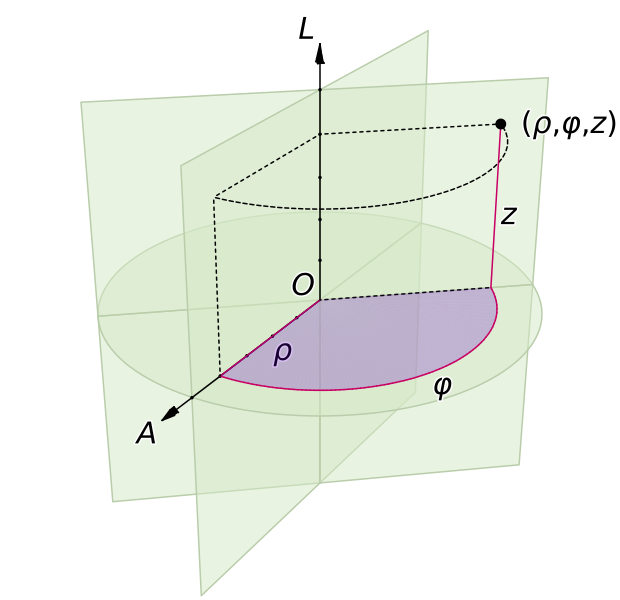
\includegraphics[width=0.8\textwidth]{figures/Coord_system_CY_1.png}
				\caption{Współrzędne cylindryczne. Źródło: Wikipedia -- Cylindrical coordinate system.
				\textcolor{red}{UWAGA:} $\rho$ na rysunku oznacza $r$ we wzorach na slajdzie.}
				\label{fig:coord_cylindrical}
			\end{figure}
		\end{column}
	\end{columns}
\end{frame}

\begin{frame}{Równania Naviera-Stokesa 4}
	\begin{columns}
	\begin{column}{0.6\textwidth}
		Prrzy czym we współrzędnych cylindrycznych:

		\begin{equation}
			(\textbf{u}\nabla)f = u_r \frac{\partial f}{\partial r} +
			\frac{u_\varphi}{r}\frac{\partial f}{\partial \varphi} +
			u_z \frac{\partial f}{\partial z}
			\label{eq:convective_cyl}
		\end{equation}

		\begin{equation}
			\Delta f = \frac{1}{r}\frac{\partial}{\partial r}\left(r
			\frac{\partial f}{\partial r}\right) +
			\frac{1}{r^2}\frac{\partial^2 f}{\partial \varphi^2} +
			\frac{\partial^2 f}{\partial z^2}
			\label{eq:laplace_cyl}
		\end{equation}
	\end{column}

	\begin{column}{.40\textwidth}
			\begin{figure}[ht]
				\centering
				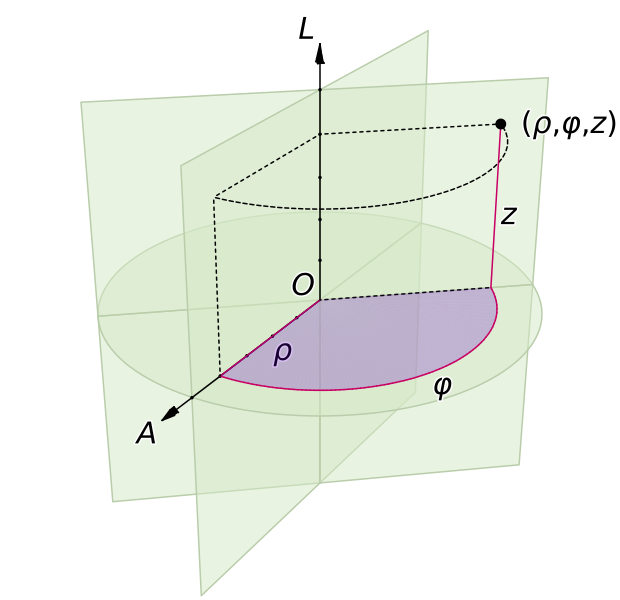
\includegraphics[width=0.8\textwidth]{figures/Coord_system_CY_1.png}
				\caption{Współrzędne cylindryczne. Źródło: Wikipedia -- Cylindrical coordinate system.
				\textcolor{red}{UWAGA:} $\rho$ na rysunku oznacza $r$ we wzorach na slajdzie.}
				%\label{fig:coord_cylindrical}
			\end{figure}
		\end{column}
	\end{columns}
\end{frame}

\begin{frame}{Równania Naviera-Stokesa 5}

	\begin{figure}[ht]
		\centering
		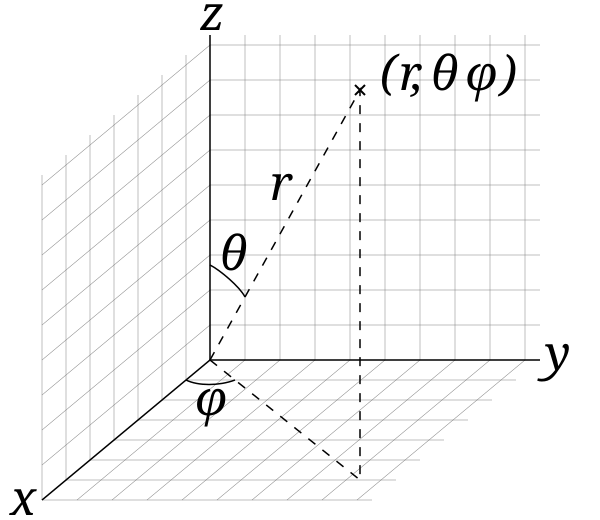
\includegraphics[width=0.65\textwidth]{figures/3D_Spherical.png}
		\caption{Współrzędne sferyczne. Źródło: Wikipedia -- Spherical coordinate system.}
		\label{fig:coord_spherical}
	\end{figure}	
\end{frame}

\begin{frame}{Równania Naviera-Stokesa 6}

	Równania Naviera-Stokesa we współrzędnych sferycznych:

	\begin{equation}
		\begin{split}
			\frac{\partial u_r}{\partial t} +
			(\textbf{u}\nabla) u_r - \frac{u_\theta^2 + u_\varphi^2}{r} =
			 -\frac{1}{\rho}\frac{\partial p}{\partial r}
			+ \\+ \nu \left(\Delta u_r - \frac{2u_r}{r^2} -
			\frac{2}{r^2 \sin \theta} \frac{\partial}{\partial \theta}
			(u_\theta \sin \theta) -\frac{2}{r^2 \sin \theta}
			\frac{\partial u_\varphi}{\partial \varphi} \right)
		\end{split}
		\label{eq:part_u_r_sphere}
	\end{equation}
	
	\begin{equation}
		\begin{split}
			\frac{\partial u_\theta}{\partial t} +
			(\textbf{u}\nabla) u_\theta + \frac{u_r u_\theta - u_\varphi^2
			\cot \theta}{r} = -\frac{1}{\rho r}\frac{\partial p}{\partial \theta} +\\
			+ \nu \left(\Delta u_\theta + \frac{2}{r^2} \frac{\partial u_r}{\partial \theta} -
			\frac{u_\theta}{r^2 \sin^2 \theta} -
			\frac{2 \cos\theta}{r^2 \sin^2 \theta} \frac{\partial u_\varphi}{\partial \varphi}
			\right)
		\end{split}
		\label{eq:part_u_theta_sphere}
	\end{equation}

	\begin{equation}
		\begin{split}
			\frac{\partial u_\varphi}{\partial t} +
			(\textbf{u}\nabla) u_\varphi + \frac{u_r u_\varphi + u_\theta u_\varphi
			\cot \theta}{r} = -\frac{1}{\rho r }\frac{\partial p}{\partial \varphi} +\\
			+ \nu \left(\Delta u_\varphi + \frac{2}{r^2 \sin \theta} \frac{\partial u_r}{\partial \varphi} +
			\frac{2 \cos \theta}{r^2 \sin^2 \theta} \frac{\partial u_\theta}{\partial \varphi} -
			\frac{u_\varphi}{r^2 \sin^2 \theta} \right)
		\end{split}
		\label{eq:part_u_phi_sphere}
	\end{equation}
\end{frame}

\begin{frame}{Równania Naviera-Stokesa 7}
	Przy czym we współrzędnych sferycznych:

	\begin{equation}
		(\textbf{u}\nabla)f = u_r \frac{\partial f}{\partial r} +
		\frac{u_\theta}{r}\frac{\partial f}{\partial \theta} +
		\frac{u_\varphi}{r \sin \theta} \frac{\partial f}{\partial \varphi}
	\label{eq:convective_sphere}
	\end{equation}

	\begin{equation}
		\begin{split}
			\Delta f = \frac{1}{r^2}\frac{\partial}{\partial r}\left(r^2
			\frac{\partial f}{\partial r}\right) +
			\frac{1}{r^2 \sin \theta} \frac{\partial}{\partial \theta}
			\left(\sin \theta \frac{\partial f}{\partial \theta}\right) +
			 \frac{1}{r^2 \sin^2 \theta} \frac{\partial^2 f}{\partial \varphi^2}
		\end{split}
	\label{eq:laplace_sphere}
	\end{equation}
\end{frame}

\begin{frame}{Szczególne przypadki 1}
	Jednym z najczęściej rozważanych przypadków przepływu płynu lepkościowego
	z wykorzystaniem równań Naviera-Stokesa jest przepływ laminarny płynu
	nad jedną płaską powierzchnią. W tym przypadku wektor prędkści 
	\textbf{u} pryzmuje postać:

	\begin{equation}
		\textbf{u} = \begin{pmatrix}
		u(y,t) \\
		0 \\
		0
		\end{pmatrix}
		\label{eq:1stex_vel}
	\end{equation}

	Według takiej postaci wektora prędkości równanie Naviera-Stokesa \eqref{eq:navier_stokes_incompressible}
	przyjmują postać:

	\begin{equation}
		\begin{split}
		\frac{\partial u}{\partial t} = -\frac{1}{\rho} \frac{\partial p}{\partial x} +
		\nu \frac{\partial^2 u}{\partial y^2}, \\
		\frac{\partial p}{\partial y} = \frac{\partial p}{\partial z} = 0
		\end{split}
	\end{equation}
\end{frame}

\begin{frame}{Szczególne przypadki 2}
	\begin{columns}

	\begin{column}{.7\textwidth}
	Innym często rozważanym przypadkiem jest stacjonarny przepływ laminarny płynu lepkiego
	na równi pochylonej pod pewnym kątem $\alpha$ do poziomu i pod wpływem grawitacji 
	\textbf{g}. W tym przypadku ogólnie wektor prędkości jest dany wyrażeniem:

	\begin{equation}
		\textbf{u} = \begin{pmatrix}
		u(y) \\
		v(y) \\
		0
		\end{pmatrix}
		\label{eq:2ndex_vel}
	\end{equation}

	Też jest ważnym że:

	\begin{equation}
		\textbf{u}(y=0) = \textbf{0}
		\label{eq:2ndex_u_y0}
	\end{equation}

	Nieścisłość mówi że:

	\begin{equation}
		\frac{dv}{dy} = 0 => v = \text{const}
		\label{eq:2ndex_y_velocity}
	\end{equation}
	\end{column}

	\begin{column}{.3\textwidth}
	\begin{figure}[ht]
		\centering
		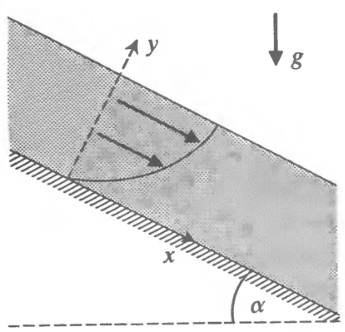
\includegraphics[width=.95\textwidth]{figures/rownPoch.png}
		\caption{Ilustracja przypadku. Źródło: D.J. Acheson -- "Elementary Fluid Dynamics",
		Cambridge University Press, 2005}
		\label{fig:rownia_pochyla}
	\end{figure}
	\end{column}

	\end{columns}

\end{frame}

\begin{frame}{Szczególne przypadki 3}
	Warunki \eqref{eq:2ndex_u_y0} i \eqref{eq:2ndex_y_velocity} dają że:

	\begin{equation}
		v = 0 = \text{const}
	\label{eq:2ndex_y_velocity2}
	\end{equation}

	Więc wektor prędkości przyjmuje postać:

	\begin{equation}
		\textbf{u} = \begin{pmatrix}
		u(y) \\
		0 \\
		0
		\end{pmatrix}
	\label{eq:2ndex_vel2}
	\end{equation}

\end{frame}

\begin{frame}{Szczególne przypadki 4}

	Podstawiając taką prędkość do równań Naviera-Stokesa \eqref{eq:navier_stokes_incompressible}
	razem z polem grawitacji można otrzymać:

	\begin{equation}
		\begin{split}
			0 = -\frac{1}{\rho} \frac{\partial p}{\partial x} & +\nu \frac{d^2u}{dy^2}  + g \sin \alpha\\
			0 = -\frac{1}{\rho} \frac{\partial p}{\partial y}  & - g \cos \alpha
			\end{split}
		\label{eq:2ndex_navier-stokes}
	\end{equation}

	Całkując drugie równanie \eqref{eq:2ndex_navier-stokes} mamy:

	\begin{equation}
		p = -\rho g y \cos \alpha + f(x)
	\label{eq:2ndex_pressure_undefined}
	\end{equation}

	Najczęściej przyjmuję się że:

	\begin{equation}
		p=p_0, \quad \mu\frac{du}{dy} = 0\ \text{przy}\ y=h - \text{swobodna powierzchnia}
	\label{eq:2ndex_pressure_bc}
	\end{equation}
\end{frame}

\begin{frame}{Szczególne przypadki 5}
	Stąd:
	
	\begin{equation}
		p - p_0 = \rho g (h-y) \cos \alpha
	\label{eq:2ndex_pressure_defined}
	\end{equation}

	Jest widocznie, że $p\neq p(x)$, więc równanie \eqref{eq:2ndex_navier-stokes}
	redukuje sie do:

	\begin{equation}
		\nu \frac{d^2u}{dy^2} = -g \sin \alpha
	\label{eq:2ndex_navier-stokes_reduced}
	\end{equation}
	
	Z warunków:

	\begin{equation}
		u(y=o) = 0, \quad \mu \frac{du}{dy}_{y=h} = 0
	\label{eq:2ndex_velocity_bc}
	\end{equation}

	Mamy rozwiązanie:

	\begin{equation}
		u(y) = \frac{g}{2\nu} y (2h-y) \sin \alpha
	\label{eq:2ndex_velocity_solution}
	\end{equation}
\end{frame}

\begin{frame}{Zastosowania 1}
	\begin{columns}
		\begin{column}{.65\textwidth}
			Z równań Naviera-Stokesa są wyprowadzane równania płytkiej 
		wody (eng: shallow water equations), które są używane do opisu
		fal na powierzchni wody, fal tsunami, itp.:

		\begin{equation}
			\begin{split}
				\frac{\partial (\rho\eta)}{\partial t} + \nabla \cdot (\rho\eta \textbf{u}) = 0 \\
				\frac{\partial(\rho\eta u)}{\partial t} + \frac{\partial}{\partial x}\left( \rho \eta u^2 + \frac{1}{2} \rho g \eta^2 \right) + \frac{\partial(\rho\eta uv)}{\partial y} = 0 \\
				\frac{\partial(\rho\eta v)}{\partial t} + \frac{\partial}{\partial y}\left( \rho \eta v^2 + \frac{1}{2} \rho g \eta^2 \right) + \frac{\partial(\rho\eta uv)}{\partial x} = 0
			\end{split}
		\end{equation}
		\end{column}

	\begin{column}{.35\textwidth}
		\begin{figure}[ht]
			\centering
			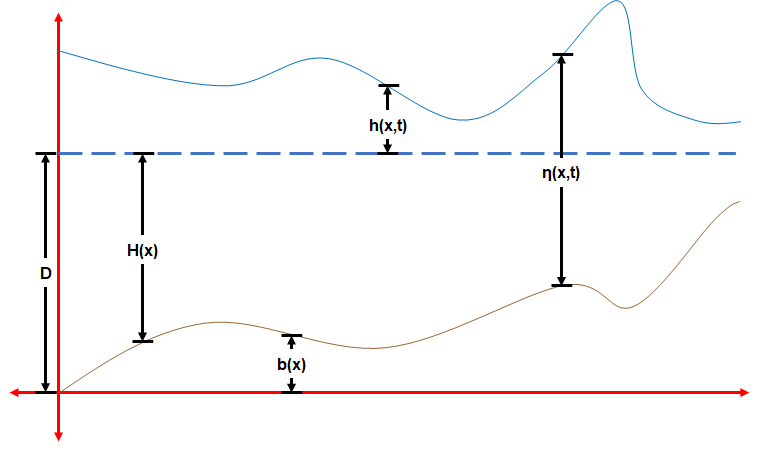
\includegraphics[width=.95\textwidth]{figures/Shallow_water_model_diagram.png}
			\caption{Ilustracja diagramu dla równań płytkiej wody. Źródło: Wikipedia -- Shallow water equations.}
			\label{fig:shallow_water}
		\end{figure}
	\end{column}
	\end{columns}
\end{frame}

\begin{frame}{Zastosowania 2}

	Biorąc jako pole zewnętrzne siłę Lorentza i dopełniając równania Naviera-Stokesa
	równaniami Maxwella można otrzymać równania tzw. elektromagnetohydrodynamiki , które są używane do opisu plazmy i gazu międzygwiezdnego, itp.:

	\begin{columns}
		\begin{column}{.5\textwidth}
			\begin{figure}
				\centering
				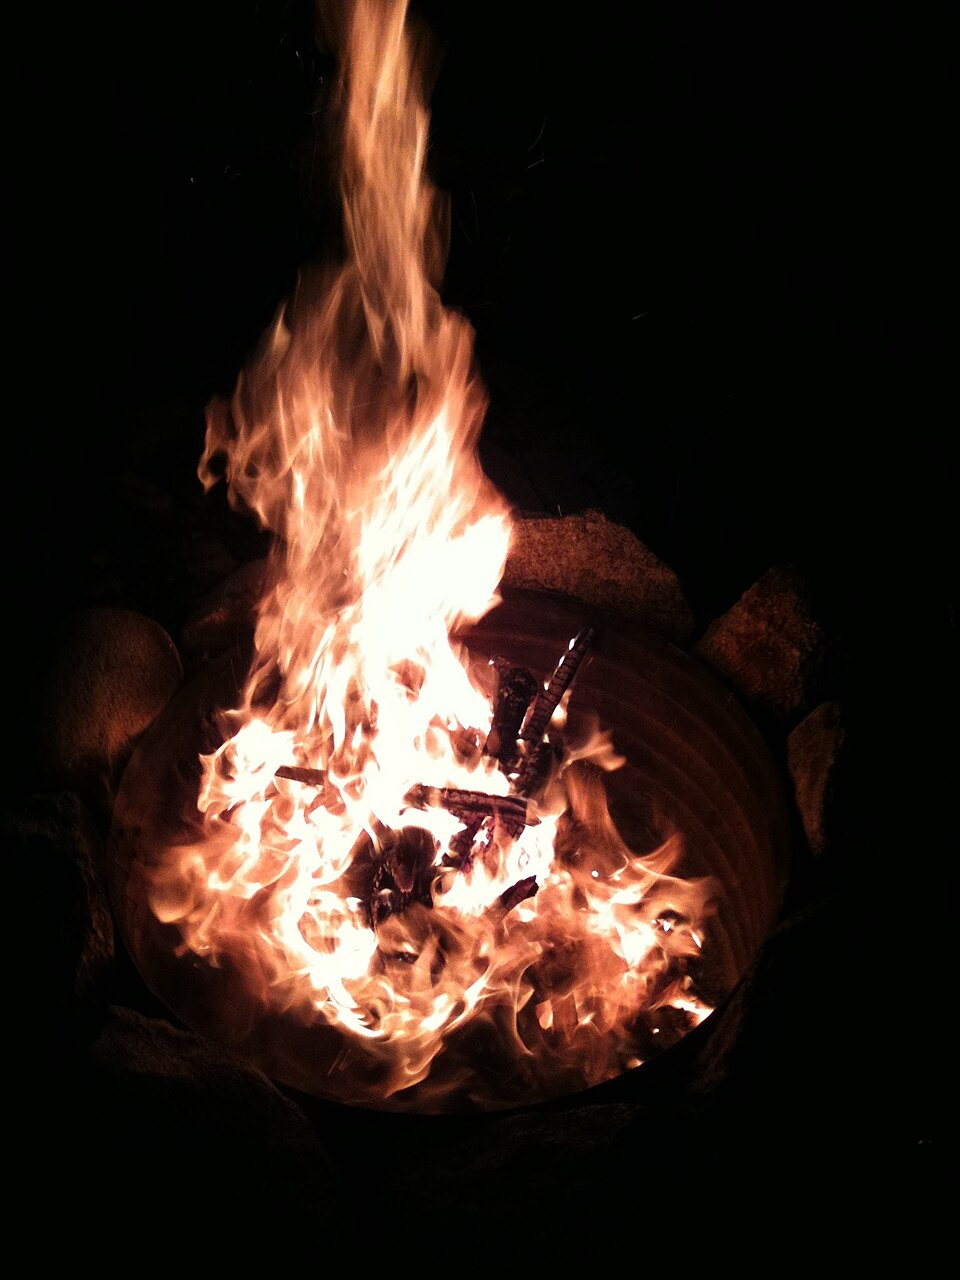
\includegraphics[width=0.5\textwidth]{figures/fire.jpg}
				\caption{Ilustracja plazmy w postaci ognia. Źródło: Wikipedia -- Plasma (physics).}
				\label{fig:plasma_fire}
			\end{figure}
		\end{column}
		\begin{column}{.5\textwidth}
			\begin{figure}
				\centering
				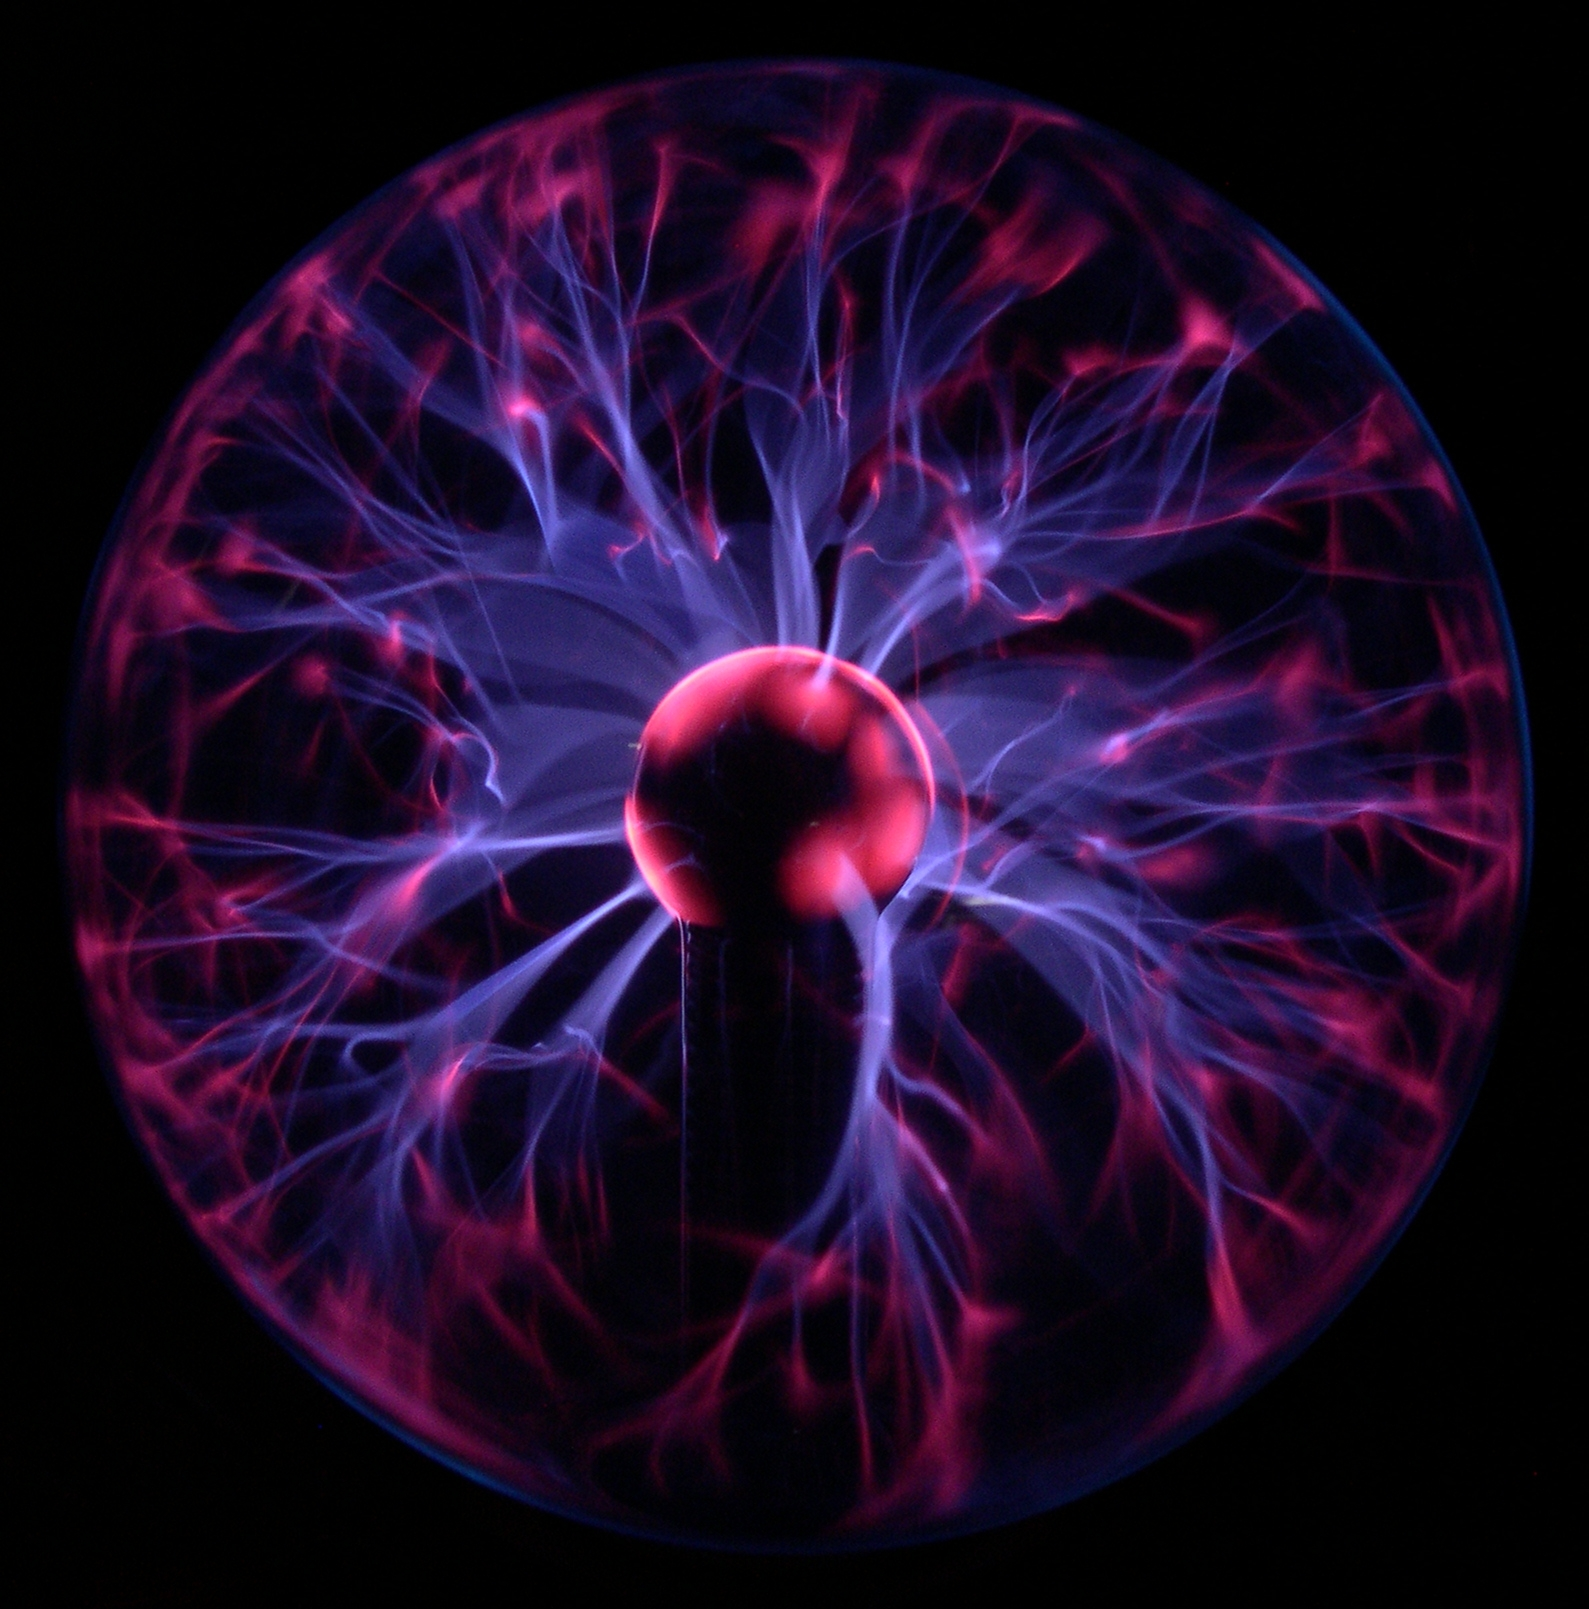
\includegraphics[width=0.5\textwidth]{figures/ball.jpeg}
				\caption{Ilustracja plazmy w postaci kuli plazmowej. Źródło: Wikipedia -- Plasma (physics).}
				\label{fig:plasma_ball}
			\end{figure}
		\end{column}
	\end{columns}
\end{frame}

\begin{frame}{Zastosowania 3}
	Dopełniając równania Naviera-Stokesa równaniami przepływów ciepła
	można modelować zjawisko konwekcji.
	
	\begin{figure}
		\centering
		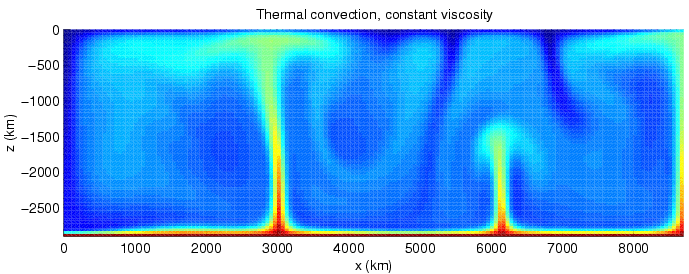
\includegraphics[width=1\textwidth]{figures/covection.png}
		\caption{Ilustracja zjawiska konwekcji w płaszczu Ziemi. Źródło: Wikipedia -- Convection (heat transfer).}
		\label{fig:convection}
	\end{figure}
\end{frame}

\begin{frame}{Zastosowania 4}
	\begin{columns}
		\begin{column}{.75\textwidth}
			Równania Naviera-Stokesa są też użyteczne w meteorologii, oceanografii.

			\begin{figure}[ht]
				\centering
				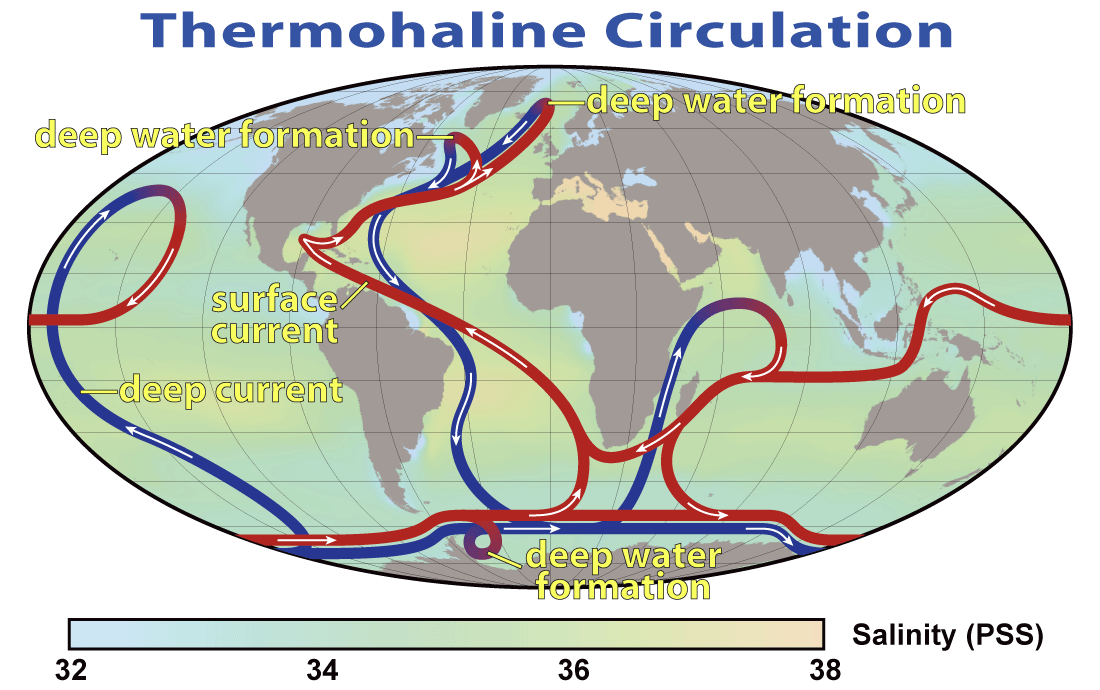
\includegraphics[width=.75\textwidth]{figures/Thermohaline_Circulation_2.png}
				\caption{Ilustracja cyrkulacji termohalinowej. Źródło: Wikipedia -- Oceanography.}
				\label{fig:thermohaline_circulation}
			\end{figure}
		\end{column}
		\begin{column}{.25\textwidth}
			\begin{figure}[ht]
				\centering
				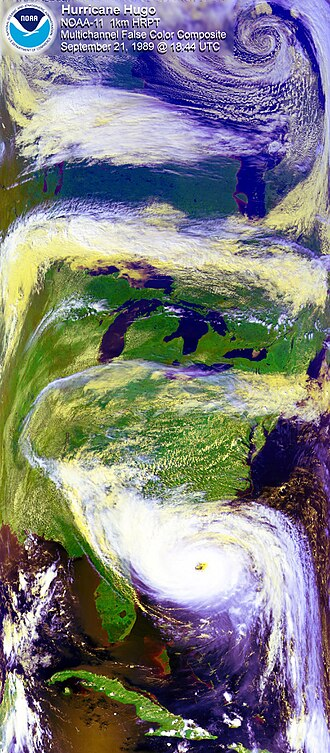
\includegraphics[width=.75\textwidth]{figures/Huracn_Hugo.jpg}
				\caption{Ilustracja huraganu Hugo. Źródło: Wikipedia -- Meteorology.}
				\label{fig:hurricane_hugo}
			\end{figure}
		\end{column}
	\end{columns}
	
\end{frame}

\begin{frame}{Zastosowania 5}
	Równania Naviera-Stokesa są kluczowe w aerodynamice i związanych z nią
	dziedzinach takich jak lotnictwo, inżynieria samochodowa, kosmonautyka, itp.
	Te równania są najczęściej używane do modelowania przepływów turbulentnych.
	\begin{columns}
		\begin{column}{.5\textwidth}
			\begin{figure}[ht]
				\centering
				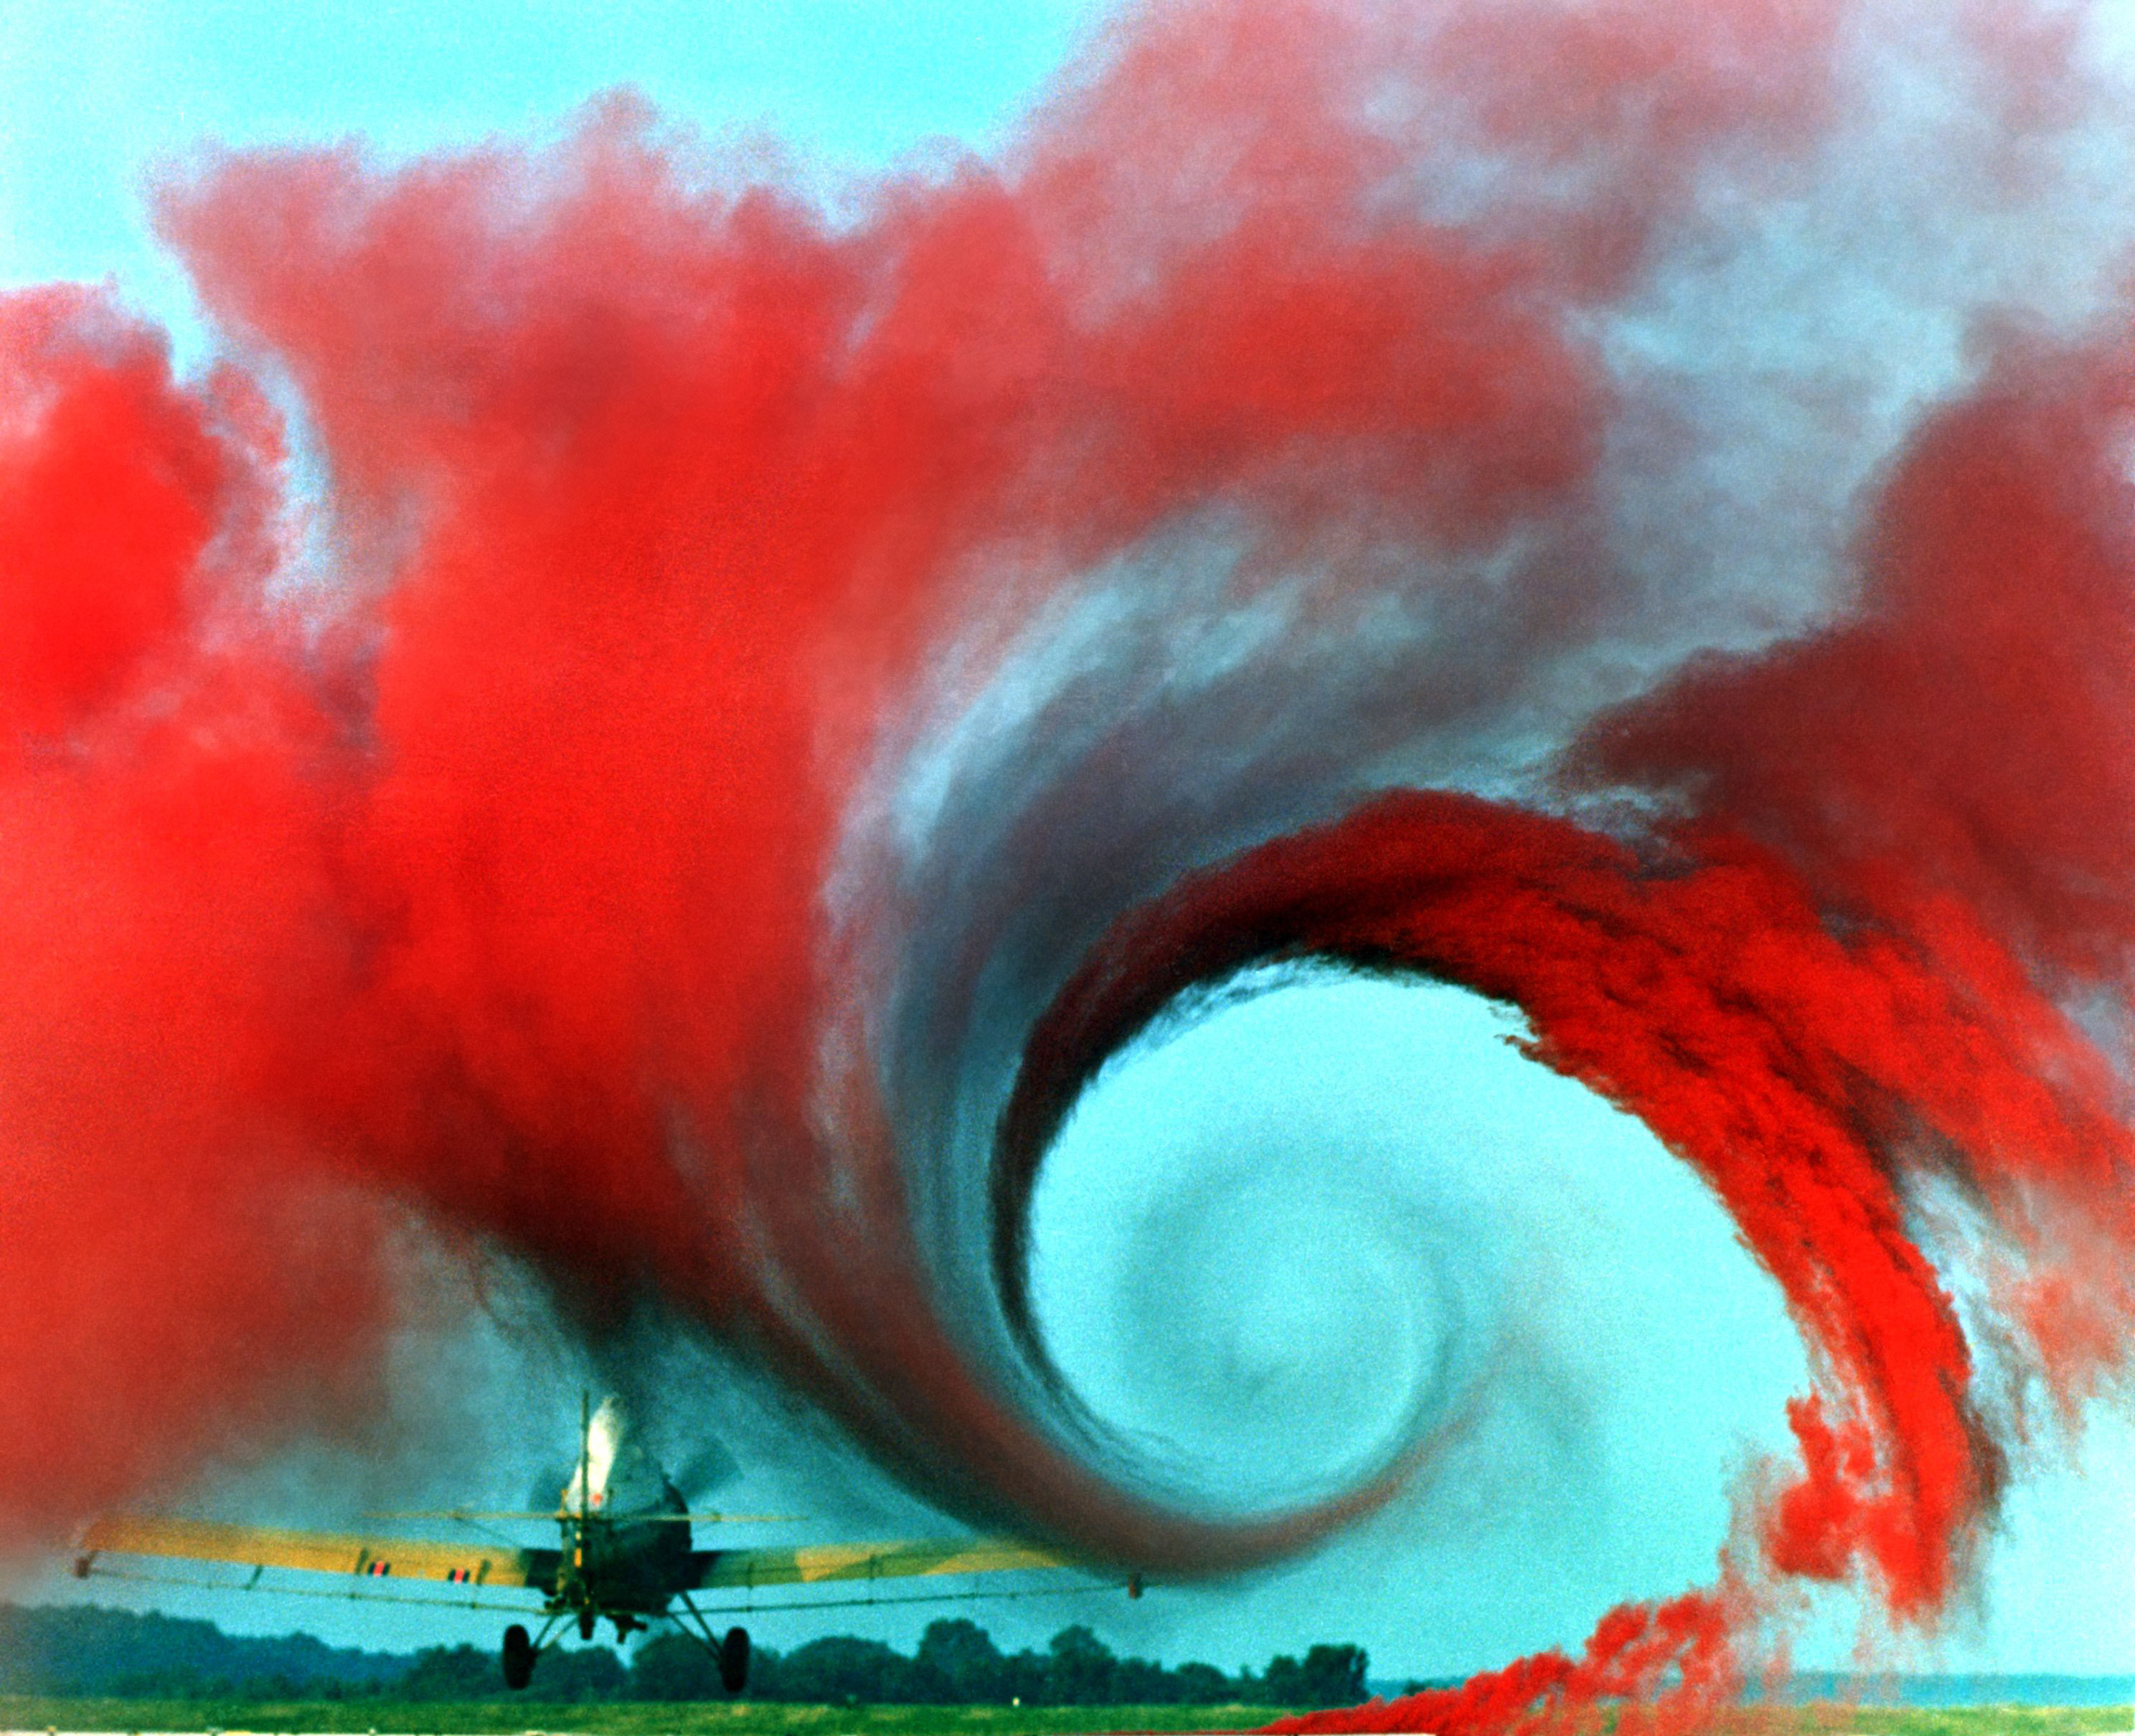
\includegraphics[width=.75\textwidth]{figures/turbo.jpeg}
				\caption{Ilustracja zjawiska turbulencji. Źródło: Wikipedia -- Turbulence.}
				\label{fig:turbulence}
			\end{figure}
		\end{column}
		\begin{column}{.5\textwidth}
			\begin{figure}[ht]
				\centering
				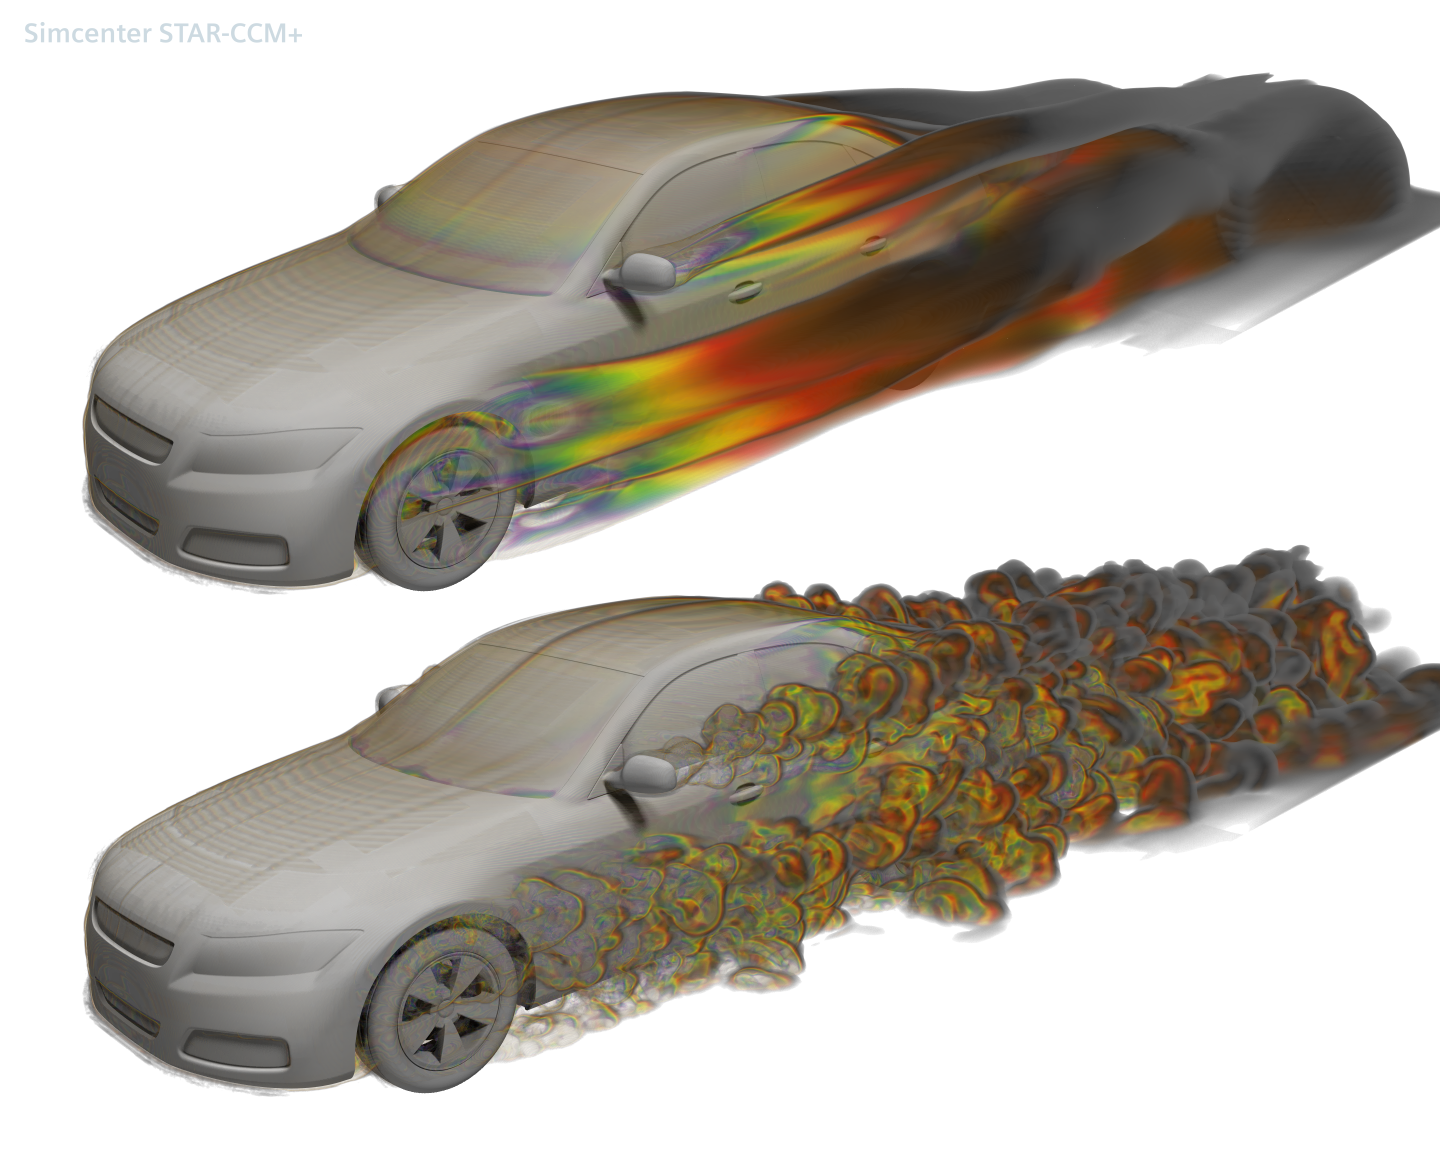
\includegraphics[width=.75\textwidth]{figures/turboModels.png}
				\caption{Ilustracja dwóch modeli obliczeniowych zjawiska turbulencji. Źródło: Wikipedia -- Computational fluid dynamics.}
				\label{fig:turbulence}
			\end{figure}
		\end{column}
	\end{columns}	
\end{frame}

\begin{frame}{Podsumowanie}
	W trakcie prezentacji zostały omówione:
	\begin{itemize}
		\item Podstawy mechaniki płynów, potrzebne do zrozumienia i wyprowadzenia
		równań Naviera-Stokesa
		\item Fizyczne i matematyczne podstawy wyprowadzenia równań Naviera-Stokesa
		\item Równania Naviera-Stokesa i ich formy przy konkretnych założeniach i w
		różnych układach współrzędnych
		\item Szczególne przypadki równań Naviera-Stokesa i ich rozwiązania
		\item Zastosowania i znaczenie równań Naviera-Stokesa w różnych dziedzinach nauki i techniki 
	\end{itemize}
\end{frame}

\begin{frame}{Źródła 1}
	Książki:
	\begin{itemize}
		\item L.D. Landau, E.M. Lifshitz -- "Gidrodinamika: Teoreticheskaya fizika, t.6", Moskva: Nauka, 1986
		\item O. Gonzales, A.M. Stuart -- "A first course in continuum mechanics", Cambridge University Press, 2008
		\item D.J. Acheson -- "Elementary Fluid Dynamics", Cambridge University Press, 2005
		\item N.E. Kochin, I.A. Kibel --
		"Teoreticheskaya gidrodinamika" ch. 1 i 2, Moskva Fizmatlit, 1963
	\end{itemize}
\end{frame}

\begin{frame}{Źródła 2}
	Linki:
	\begin{itemize}
		\item Wikipedia -- Navier-Stokes equations:
		\url{https://en.wikipedia.org/wiki/Navier-Stokes_equations}

		\item Wikipedia -- Euler equations (fluid dynamics):\\
		\url{https://en.wikipedia.org/wiki/Euler_equations_(fluid_dynamics)}

		\item Wikipedia -- Cylindrical coordinate system:
		\url{https://en.wikipedia.org/wiki/Cylindrical_coordinate_system}

		\item Wikipedia -- Spherical coordinate system:
		\url{https://en.wikipedia.org/wiki/Spherical_coordinate_system}

		\item Wikipedia -- Shallow water equations:
		\url{https://en.wikipedia.org/wiki/Shallow_water_equations}
	\end{itemize}
\end{frame}

\begin{frame}{Źródła 3}
	Linki (c.d.):
	\begin{itemize}
		\item Wikipedia -- Plasma (physics):
		\url{https://en.wikipedia.org/wiki/Plasma_(physics)}

		\item Wikipedia -- Convection (heat transfer):
		\url{https://en.wikipedia.org/wiki/Convection_(heat_transfer)}

		\item Wikipedia -- Oceanography:
		\url{https://en.wikipedia.org/wiki/Oceanography}

		\item Wikipedia -- Meteorology:
		\url{https://en.wikipedia.org/wiki/Meteorology}

		\item Wikipedia -- Turbulence:
		\url{https://en.wikipedia.org/wiki/Turbulence}

		\item Wikipedia -- Computational fluid dynamics:
		\url{https://en.wikipedia.org/wiki/Computational_fluid_dynamics}
	\end{itemize}
\end{frame}


%%% PG LAST PAGE %%%
\pglastframe


%%% DOCUMENT ENDS HERE. Good bye! :) %%%

\end{document}

